\documentclass[12pt,a4paper]{article}
\usepackage{hyperref}
\usepackage{graphicx}
\usepackage{amsmath}
\title{Laboratory 3: DSSS}
\author{Niclas Scheuing and Vasileios Dimitrakis}

\newtheorem{theorem}{Observation}
	
\begin{document}
	\maketitle
	
	\section{Introduction}
	The goal of this laboratory exercise is to study the spread spectrum techniques. Spread spectrum schemes spread the signal over a large frequency band. The main idea behind this systems is to use more bandwidth and at the same time to maintain the same amount of power in the whole signal. These techniques offer increased resistance to interference, noise, jamming and channel multipath and fading effects. These properties make them very popular and frequently preferred in communication systems. 
	There are three main spread spectrum techniques that are frequently used:
	\begin{itemize}
	\item{\emph{Frequency Hop Spread Spectrum}: Is a method of transmitting radio signals by rapidly switching a carrier among many frequency channels, using a pseudorandom sequence known to both transmitter and receiver.}
	\item{\emph{Chirp}: Is a signal, which decreases or increases its frequency continuously over time. It has many applications and one of them is the property of spread spectrum that offers.}
	\item{\emph{Direct Sequence Spread spectrum}: Is a spread spectrum technique whereby the original data signal is multiplied with a pseudo random noise spreading code.}
	\end{itemize}
	
	In this exercise we will study the case of the Direct Sequence Spread Spectrum (DSSS).
	In DSSS the signal is used to modulate a bit sequence, which is known as Pseudo Noise (PN) code. This code consists of pulses that have much shorter duration than the one of original signal. Therefore, this process chops up the pulses of the message signal and this leads to broader signal's bandwidth that tends to be equal to the one of the PN code. 
	This spread spectrum technique is widely used, because it offers many benefits and for this reason, it is widely used in both military and civilian communication systems.
	
	\begin{itemize}
	\item{Resistance to intended or unintended jamming.}
	\item{Multiple users can share the same channel.}
	\item{Robust against noise.}
	\item{It provides a way to determine relative timing between transmitter and receiver.}
	\item{DSSS spreads the signal over a wide range of frequency and the latter can be hidden below noise level.}
	\end{itemize}
	
	\section{Topology}
	In this exercise we have one DSSS transmitter and one DSSS receiver. In this system, we have two main signal components: the message signal m(t) and the pseudorandom code code(t). \newline
	\textbf{Transmitter:} First of all, the transmitter modulates the data signal with a primary modulator using a modulation scheme, e.g BPSK. After that it multiplies the outcome of the previous process with the PN code generator and the bandwidth of the signal is spread to a wider range of frequencies.
	\newline
	\textbf{Receiver:} On the other hand, in the receiver the reverse process is followed. Firstly, the receiver despreads the broadened signal using the appropriate PN code. In the next step, it demodulates the signal using the carrier, in order to retrieve the data.
	
	\section{Materials and Methods}
	Throughout the lab exercise 3 we used \emph{MATLAB}, a vector- and numerical computing environment.
	
	\section{Theory}
	Some basic concepts need to be discussed first.
	\subsection{Signal analysis}
	To reason about the power spectrum of a signal $s(t)$ we need to study its Fourier transform $F(s)$.
	Let's assume $s$ consists of block functions
	\begin{equation}
		b_{\sigma, T}(t) = \left\{
		\begin{array}{ll}
			1  & \mbox{if } \sigma-\frac{T}{2} < t < \sigma+\frac{T}{2} \\
			0 & \mbox{else}
		\end{array}
		\right.
	\end{equation}
	 where $\sigma$ is the center of the block function, $T$ the width and $n$ the number of blocks. So our signal is the following
	 \begin{equation}
	 	s(t) = \sum_{i=1}^{n} b_{\sigma_i, T}(t)
	 \end{equation}.
	Looking at the Fourier transform we get	
	\begin{align}
		F(s(t)) & = \int_{-\infty}^{\infty} s(t) e^{-2i \pi t \xi} dt\\
		& = \int_{-\infty}^{\infty}  \sum_{i=1}^{n} s(t) e^{-2i \pi t \xi} dt\\
		& = \sum_{i=1}^{n} \int_{-\infty}^{\infty}  s(t) e^{-2i \pi t \xi} dt\\
		& = \sum_{i=1}^{n} \int_{t_i-\frac{T}{2}}^{t_i + \frac{T}{2}}  e^{-2i \pi t \xi} dt\\
		& = \sum_{i=1}^{n} \frac{1}{-2\pi i \xi}\left[e^{-2i \pi t \xi} \right]_{t_i - \frac{T}{2}}^{t_i + \frac{T}{2}}\\
		& = \sum_{i=1}^{n} \frac{1}{-2\pi i \xi}
		\left[e^{-2i \pi (t_i +\frac{T}{2}) \xi} - e^{-2i \pi (t_i -\frac{T}{2}) \xi}\right]\\
		& = \sum_{i=1}^{n} \frac{1}{-2\pi i \xi}
		\left[e^{-2i \pi t_i \xi} e^{-i \pi T \xi} - e^{-2i \pi t_i  \xi} e^{i \pi T \xi} \right]\\
		& = \sum_{i=1}^{n} e^{-2i \pi t_i \xi} \frac{1}{\pi \xi}
		  \left[ \frac{e^{-i \pi T \xi} - e^{i \pi T \xi}}{-2i} \right]\\
		& = \sum_{i=1}^{n} e^{-2i \pi t_i \xi} \frac{T}{T \pi \xi} \sin(\pi T \xi)\\
		& = \sum_{i=1}^{n} e^{-2i \pi t_i \xi} T \mbox{sinc}(T \xi)\\
	\end{align}
	
	The power spectrum is the $s(t)$ is the function $\left| F(s)\right|$, which yields
	\begin{equation}
		\left|F(s)\right| = \left| \sum_{i=1}^{n} e^{-2i \pi t_i \xi} T \mbox{sinc}(T \xi) \right| = T  \sum_{i=1}^{n} \left| \mbox{sinc}(T \xi) \right|
	\end{equation}
	
	
	There are two main observations to be made.
	\begin{theorem}\label{maximum}
		The maximum of the power spectrum of a block shape signal $s(t)$ is proportional to the width of one block $T$.
	\end{theorem}
	\begin{theorem}\label{lobe}
		The width of the first lobe of the power spectrum of a block function $b_{t_0,T}(t)$ is proportional to $\frac{1}{T}$.
		More formally: $2\left| t-t_0 \right| \propto \frac{1}{T}$ where $t_0$ is the center of the block function and for $t$ holds $b_{t_0,T}(t) = 0$ and $\left|t -t_0\right|$ is minimal.
	\end{theorem}
	
	\subsection{Processing gain}
	In a spread spectrum system, the process gain $P$ (or 'processing gain') is the ratio of the DSSS signal bandwidth to the \texttt{data} bandwidth. It is usually expressed in decibels (dB). This is equivalent to the ratio of the maximum of the \texttt{data}'s power spectrum to the maximum of the DSSS signal's power spectrum. Observation\ref{maximum} thus yields $P = \frac{T_d}{T_c}$
	
	\section{Terminology}
	The data array, representing our block signal, is denoted as \texttt{data} and the chip sequence \texttt{chip.}
	The length on the time axis of a \texttt{data} bit is  named \texttt{$T_d$} where the length on the time axis of a \texttt{code} bit is \texttt{$T_c$}.
	
	The total length of \texttt{data} in bits is called \texttt{DL} and of the \texttt{code} \texttt{CL}.
	
	
	\section{Tasks}
		The following steps were done when working with the MATLAB implementation of DSSS.
		
		Executing it for the firsttime resulted in the despreading to fail.
		This was due to the fact that despreading with a different code than the one used for spreading, does not restore the original message.
		
		We then fixed the code and made it use the same key for spreading and despreading. The reconstruction of the DSSS 
		signal succeeded.
		

\paragraph{Configuring the DSSS system} \label{config}
	\texttt{DL} and \texttt{CL} were used in the following four configurations.
	\begin{enumerate}
		\item \texttt{DL}$=10$bit , \texttt{CL}$=10$bit. 
			See \autoref{10:10} and \autoref{ft:10:10}. \\
			\texttt{data = [1 -1 1 -1 1 -1 1 -1 1 -1]}\\
			This results in a one chip per symbol modulation, which means $T_d = T_c$ and for the processing gain $P = \frac{10}{10} = 1$ 
			Accordingly, as seen in \autoref{ft:10:10}, the power spectra of \texttt{data} and the DSSS signal is almost the same.
			
		\item \texttt{DL}$=10$bit , \texttt{CL}$=100$bit. 
			See \autoref{100:10} and \autoref{ft:100:10}. \\
			\texttt{data = [1 -1 1 -1 1 -1 1 -1 1 -1]}\\
			$P = \frac{100}{10} = 10$. By looking at the plots, we observed a processing gain that is rather 3.5. The calculated value is for a block signal and the measurements were made on a BPSK modulated signal. The observed deviations might root in this difference.\\
			\autoref{ft:100:10} shows that the power spectra of \texttt{data} is much smaller than the the DSSS signal's because \texttt{$T_c$} $<<$ \texttt{$T_d$}.
		
		\item \texttt{DL}$=5$bit , \texttt{CL}$=100$bit. 
			See \autoref{100:5} and \autoref{ft:100:5}. \\
			\texttt{data = [1 -1 1 -1 1 ]}\\
			$P=\frac{100}{5} = 20$. The same observation as previously are made.\\
			The power spectra seen in \autoref{ft:100:5} look almost the same as for \texttt{DL}=10 and \texttt{CL} = 100. The \texttt{data} power spectrum for \texttt{DL}=5 is slightly lower than for \texttt{DL}=10 since \texttt{$T_{d_5}$} $>$ \texttt{$T_{d_{10}}$}
			The  DSSS signal power spectrum is very similar since the \texttt{$T_c$} does not change.
		
		\item When using \texttt{DL}=5 and \texttt{CL} = 300 we observe some weird behavior in the MATLAB implementation. We assume this is a bug. See \autoref{300:10}.
	\end{enumerate}

	
	
	\section{Questions}
		
		\subsection{Jamming resistance of DSSS}\label{jamming}
		The broadband signaling schemes are more difficult to jam, because their energy is spread through a broad span of frequencies. The receiver has the same spreading code that the transmitter used to spread the signal and he is able to retrieve the message. 
		
		\paragraph{Narrow-band jamming} Resistant, because the jamming signal gets spread while despreading.
		
		\paragraph{Wide-band} Resistant because the jamming signal is not correlated to code and thus does not get despread. Except if the jamming power is high enough to cover the despread signal.

\subsection{Security introduced by DSSS}
	The CIA security properties and the possibility to detect a DSSS signal under noise are discussed in this section.
		
	\paragraph{Confidentiality}
	In a noise-less setup DSSS does not provide IND-CPA, because it is deterministic. An chosen plaintext attack will immediately reveal the code when the plaintext message gets XORed to the ciphertext.
	The DSSS signal looks random to anyone not knowing the code. In presence of noise the signal is said to be \emph{hidden below the noise}. An eavesdropper can not distinguish between the noise and the DSSS signal.
	But this still does not provide IND-CPA, since noise has some statistical properties that can be used filtering. Also the position in time can just be brute-forced by multiplying the observed DSSS signal with the plaintext message using different time shifts.
	
	\paragraph{Integrity}
	DSSS does not provide strong integrity.
	Th receiver cannot verify that the message has not been altered by an attacker or a very unlucky noise constellation.
	
	\paragraph{Availability}
	DSSS does assure availability in presence of a jammer as discussed in \autopageref{jamming}.
	
	\paragraph{Detection} \cite{power}
	In the presence of noise a DSSS signal is hard to detect. It has some static properties that make it distinguishable from random noise, such as a constant chip length, though. Also by monitoring the energy level of the electro magnetic waves, the presence of an additional sender can be revealed.
	
\subsection{Advantages and uses of DSSS}
	Beyond the property of avoiding intended or unintended jamming and the other security properties that DSSS provides, it has also some other uses and advantages\cite{wiki:dsss}:
	
	\begin{itemize}
		
		\item{First of all, the United States GPS, the European Galileo and the Russian GlONASS satellite navigation systems use DSSS, when they transmit their data, as they can share the same channel for multiple users using different codes.}
		
		\item{DS-CDMA is a multiple access scheme based on DSSS, by spreading the signals from/to different users with different codes.}
		
		\item{Cordless phones operating in 900 MHz, 2.4 GHz and 5.8 GHz bands use DSSS.}
		
		\item{DSSS is also used for IEEE 802.11b 2.4 GHz Wi-Fi, its predecessor 802.11-1999 and for IEEE 802.15.4.}
		
	\end{itemize}
	
		\section{Analysis}
		Summarizing all above, we conclude our report with the following statements
		
		\begin{itemize}
			\item
			Observations \ref{maximum} and \ref{lobe} were clearly visible in \autoref{config}, but with some deviations. We assume these are due to using BPSK modulation instead of a block signal.
			We summarize our observations about the processing gain and the reasoning from Observation \ref{maximum} and \ref{lobe} as a dependency not on \texttt{CL} or \texttt{DL} but on the ratio $\frac{CL}{DL}$
		
			\item
			DSSS is robust against intended and unintended jamming, as it is able to hide the signal below the noise level.
			Finally, broadband jamming can be effective, if the attacker has enough power to use, in order to achieve his goal.
		
			\item Eavesdroppers cannot simply retrieve the original signal if they do not have the spreading code. Some of the basic security properties are not given though.
			
			
		\end{itemize}
		
		
		
		
%10 10
	\begin{figure}
		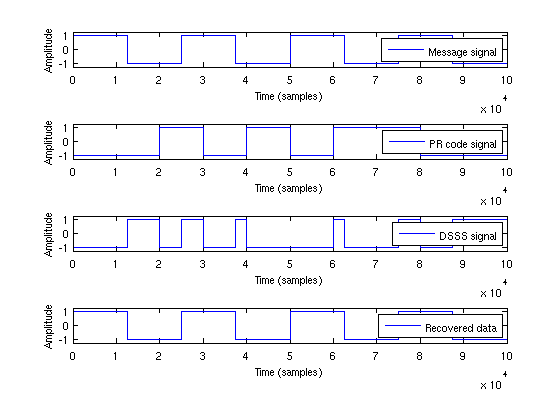
\includegraphics[width=\textwidth]{images/code_cl10_dl10.png}
		\caption{Original, spread and despread signal and code. Code length: 10bit, data length: 10bit}
		\label{10:10}
		
		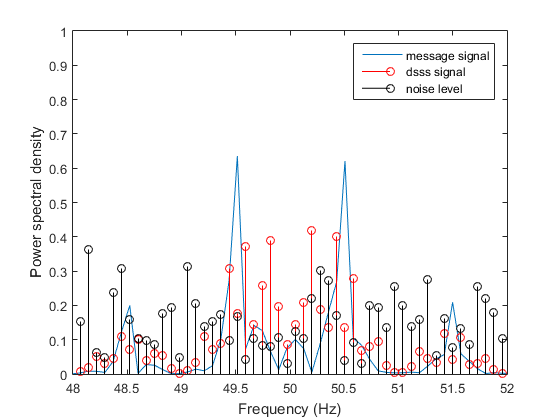
\includegraphics[width=\textwidth]{images/ft_cl_10_dl10.png}
		\caption{Original, spread and noise power spectra. Code length: 10bit, data length: 10bit}
		\label{ft:10:10}
	\end{figure}
%100 10
	\begin{figure}
		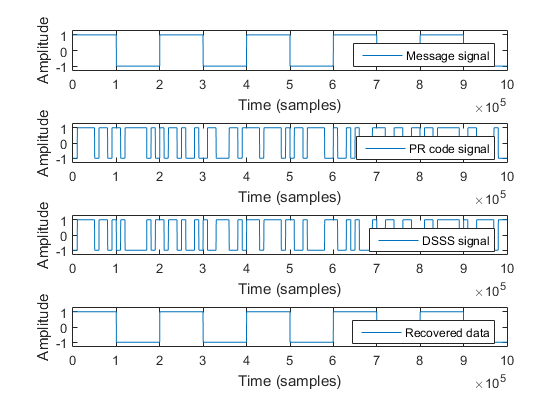
\includegraphics[width=\textwidth]{images/code_cl100_dl10.png}
		\caption{Original, spread and despread signal and code. Code length: 100bit, data length: 10bit}
		\label{100:10}
		
		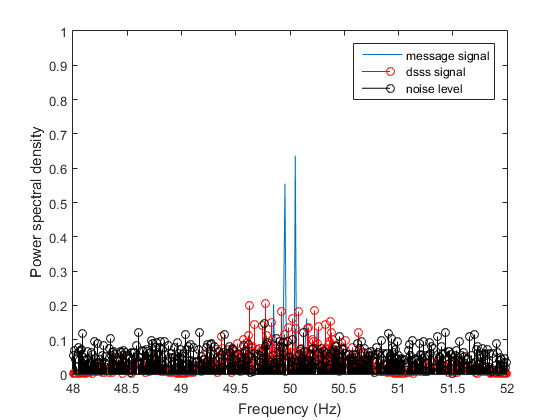
\includegraphics[width=\textwidth]{images/ft_cl_100_dl10.png}
		\caption{Original, spread and noise power spectra. Code length: 100bit, data length: 10bit}
		\label{ft:100:10}
	\end{figure}

%100 5
	\begin{figure}
		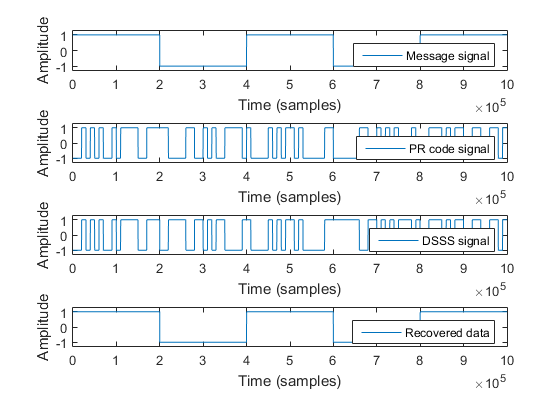
\includegraphics[width=\textwidth]{images/code_cl100_dl5.png}
		\caption{Original, spread and despread signal and code. Code length: 100bit, data length: 5bit}
		\label{100:5}
		
		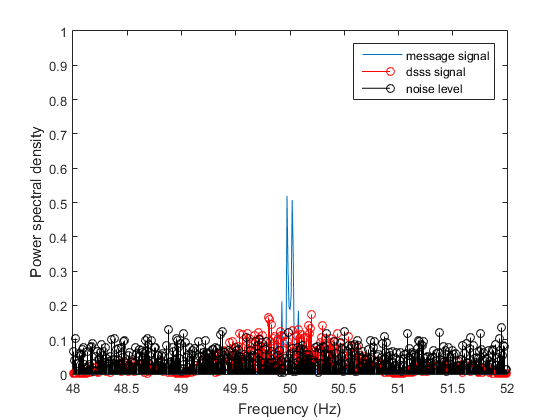
\includegraphics[width=\textwidth]{images/ft_cl_100_dl5.png}
		\caption{Original, spread and noise power spectra. Code length: 100bit, data length: 5bit}
		\label{ft:100:5}
	\end{figure}

%300 10	
	\begin{figure}
		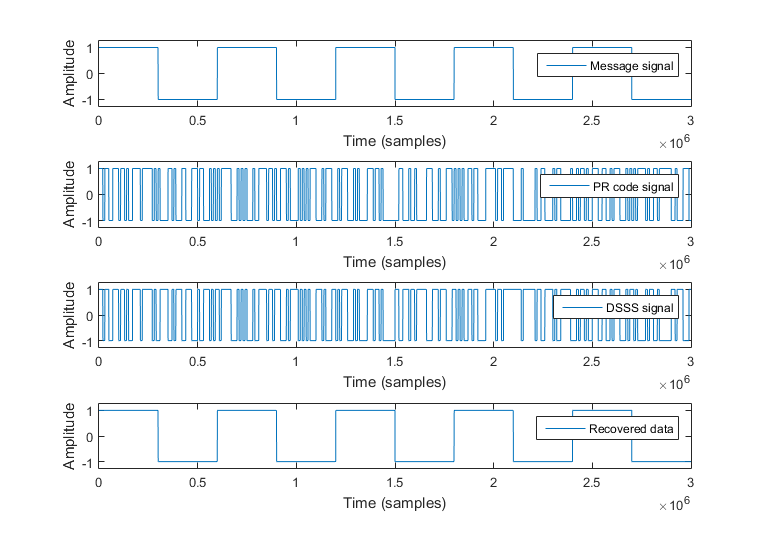
\includegraphics[width=\textwidth]{images/code_cl300_dl10.png}
		\caption{Original, spread and despread signal and code. Code length:300bit, data length: 10bit. The time axis seems to be buggy. The data array labeling is wrong.}
		\label{300:10}
		

		
%%		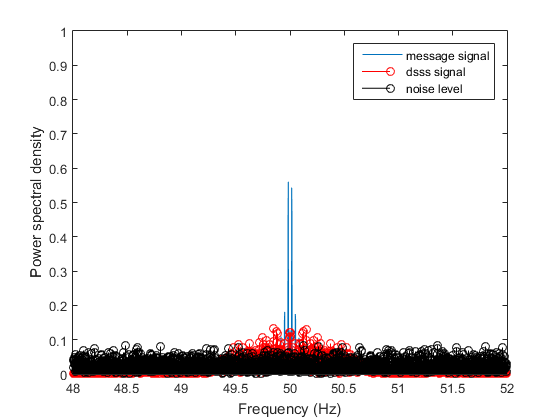
\includegraphics[width=\textwidth]{images/ft_cl_300_dl10.png}
%%		\caption{Original, spread and noise power spectra.Code length: 300bit, data length: 10bit}
%%		\label{ft:300:10}
	\end{figure}
	



	
	

	
	\bibliographystyle{plain}
	\bibliography{bibliography}
\end{document}\grid
